\newpage

% ANNEXE IHM
% ==============================================================
\sectionintro{Annexe B · Initiative personnelle}{IHM ajoutées après l'entretien}{Deux niveaux de supervision ont été développés en complément du sujet initial : une PLC Visualization V1, puis une application TwinCAT HMI V2.}
\label{annexe:ihm}

\begin{primarycard}
  \textbf{Positionnement du complément}\par\small
  L'interface opérateur ne faisait pas partie de la demande formulée pendant l'entretien. Elle a été ajoutée ensuite à titre personnel pour prolonger la démarche : rendre le cycle observable, faciliter la simulation et montrer une séparation claire entre logique PLC, communication et présentation. Cette annexe documente ce travail sans l'intégrer artificiellement au périmètre initial.
\end{primarycard}

\subsection{B.1 · PLC Visualization V1}

\begin{figure}[h]
  \centering
  \fcolorbox{ekline}{white}{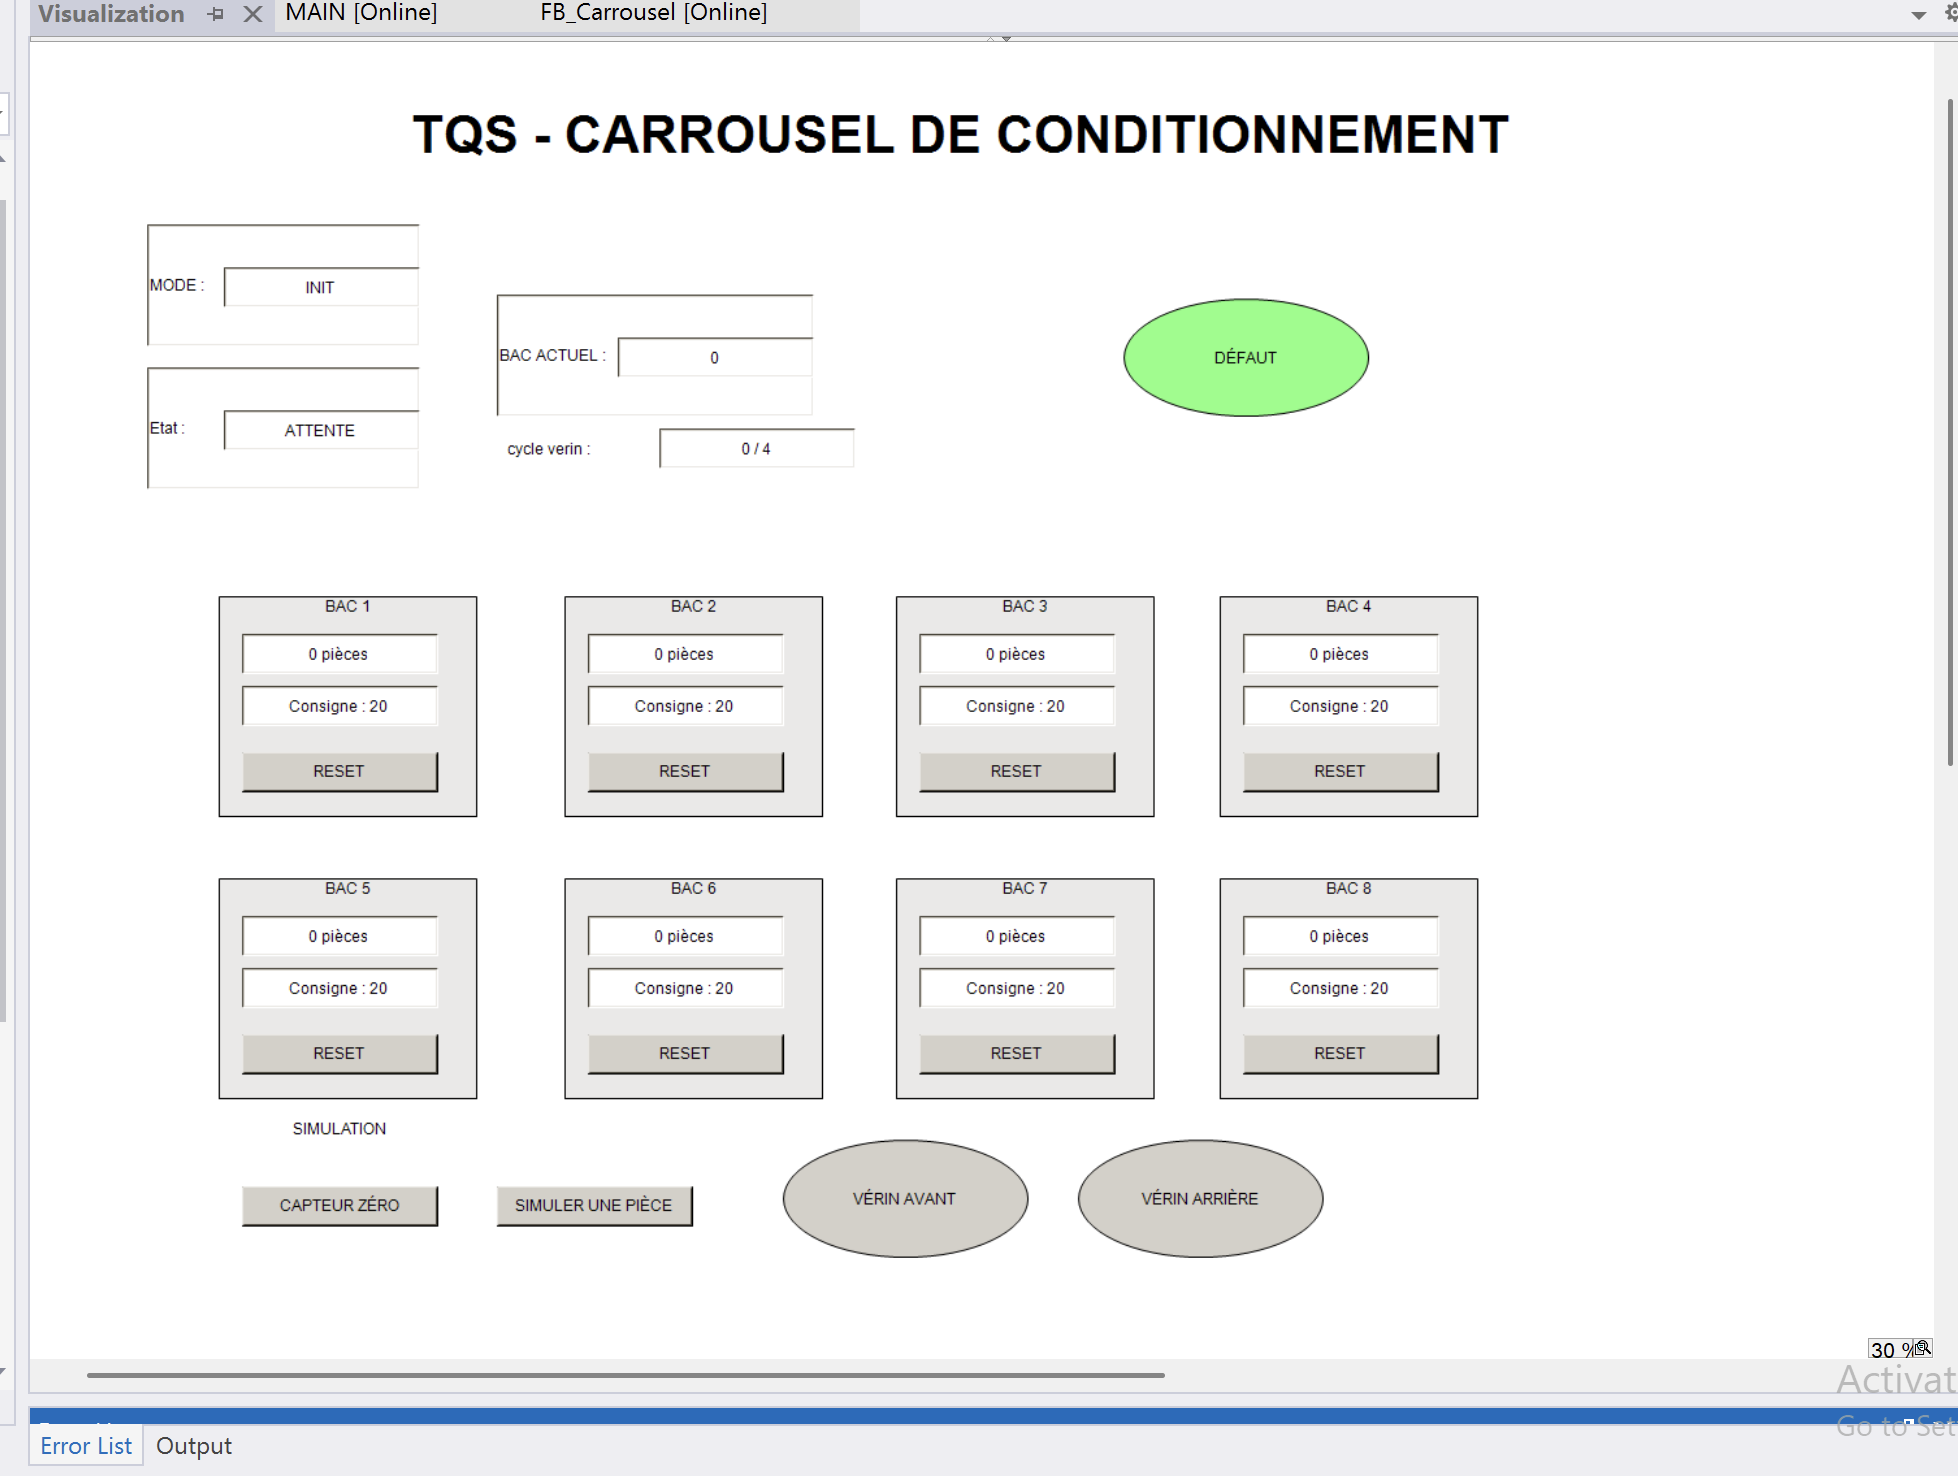
\includegraphics[width=.67\linewidth]{../images/VISU1.png}}
  \caption{PLC Visualization V1 ouverte en ligne dans TwinCAT XAE.}
\end{figure}

\vspace{-2mm}
\twocolpage{
  \begin{notebox}{Nature de l'interface}
    \small
    Cette première version est intégrée au projet automate. \texttt{Visualization.TcVIS}, son gestionnaire et la liste de textes constituent une vue locale destinée à la mise au point et à la simulation dans TwinCAT XAE.
  \end{notebox}
}{
  \begin{card}
    \textbf{Informations et commandes exposées}\par\small
    Mode, état du cycle, bac actif, compteurs des huit bacs, consigne, progression des quatre cycles vérin, défaut et commandes avant/arrière. Les boutons permettent de simuler le capteur zéro, le passage d'une pièce et la réinitialisation des bacs.
  \end{card}
}

\newpage

% ANNEXE IHM - SUITE
% ==============================================================
\sectionintro{Annexe B · Suite}{TwinCAT HMI V2}{Une seconde interface web reprend les données du PLC dans un tableau de bord plus lisible et sépare explicitement la communication ADS de l'affichage.}

\begin{figure}[h]
  \centering
  \fcolorbox{ekline}{white}{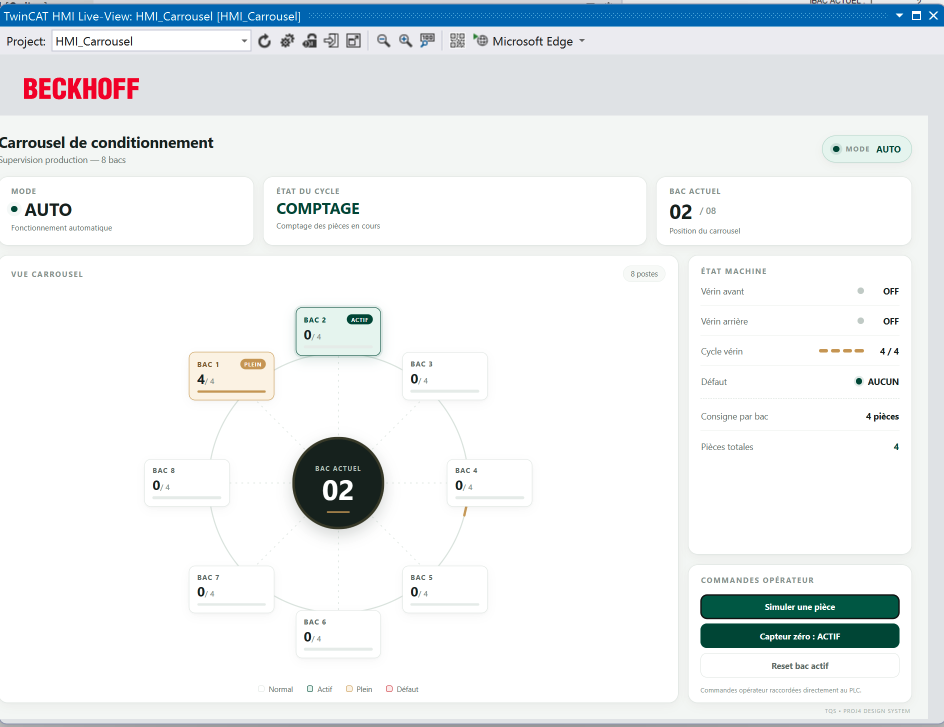
\includegraphics[width=.72\linewidth]{../images/VISU2.png}}
  \caption{TwinCAT HMI V2 dans la Live-View : bac 2 actif, bac 1 plein et cycle de comptage en cours.}
\end{figure}

\vspace{-2mm}
\twocolpage{
  \subsection{Architecture retenue}
  \begin{card}
    \small
    \texttt{PlcService} encapsule la lecture, la surveillance et l'écriture des symboles ADS. \texttt{CarouselController} coordonne les échanges. \texttt{DashboardView} met à jour l'écran et \texttt{DashboardTemplate} construit sa structure. Le fichier source \texttt{Themes/Base/TqsDashboard.css} centralise le thème graphique, les couleurs d'état et la mise en page responsive. La logique machine reste exclusivement dans le PLC.
  \end{card}
}{
  \subsection{Échanges avec le PLC}
  \begin{tabularx}{\linewidth}{@{}L{24mm}Y@{}}
    \toprule
    \textbf{Sens} & \textbf{Données}\\
    \midrule
    PLC vers IHM & mode, état, bac actif, consigne, huit compteurs, cycle vérin, commandes avant/arrière et défaut\\
    IHM vers PLC & simulation pièce, capteur zéro et reset momentané du bac actif\\
    \bottomrule
  \end{tabularx}

  \begin{notebox}[colback=ekwarning,colframe=orange!35]{Limite conservée}
    Cette interface complète la démonstration, mais ne remplace pas une IHM de production qualifiée : les alarmes historisées, la gestion des droits, la sécurité machine et le diagnostic mécanique restent hors périmètre.
  \end{notebox}
}
